\documentclass[12pt]{amsart}

% packages

\usepackage{amsfonts, amsthm, amssymb, amsmath, stmaryrd, etoolbox, mathtools}
\usepackage[margin=1in]{geometry}
\usepackage{graphicx,caption,subcaption}
\usepackage{tikz}
\usetikzlibrary{matrix,arrows}

% new commands

\newcommand{\RR}{\mathbb{R}}
\newcommand{\ZZ}{\mathbb{Z}}
\newcommand{\NN}{\mathbb{N}}
\newcommand{\QQ}{\mathbb{Q}}
\newcommand{\CC}{\mathbb{C}}
\newcommand{\from}{\colon}
%\newcommand{\defn}[1]{\textbf{#1}}
\newcommand{\tin}{\colon}

% fonts
\newcommand{\cat}[1]{\mathbf{#1}}
\newcommand{\type}[1]{\mathtt{#1}}

% types
\newcommand{\A}{\type{A}}
\newcommand{\B}{\type{B}}
\newcommand{\C}{\type{C}}
\newcommand{\BAC}{\B =_{\A} \C}
\newcommand{\Type}{\type{Type}}
\newcommand{\ap}{\type{ap}}
\newcommand{\inl}{\type{inl}}
\newcommand{\inr}{\type{inr}}
\newcommand{\glue}{\type{glue}}
\newcommand{\refl}{\type{refl}}
\newcommand{\code}{\type{code}}
\newcommand{\encode}{\type{encode}}
\newcommand{\decode}{\type{decode}}


% math operators
\DeclareMathOperator{\Hom}{Hom}
\DeclareMathOperator{\id}{id}
\DeclareMathOperator{\ob}{Ob}
\DeclareMathOperator{\arr}{arr}
\DeclareMathOperator{\im}{im}
\DeclareMathOperator{\Aut}{Aut}
\DeclareMathOperator{\Bij}{Bij}
\DeclareMathOperator{\Sub}{Sub}

% theorem styles
\newtheorem{lemma}{Lemma}
\newtheorem{thm}{Theorem}
\newtheorem{prop}{Proposition}
\newtheorem{cor}{Corollary}
\theoremstyle{remark}
\newtheorem{rmk}{Remark}
\theoremstyle{definition}
\newtheorem{defn}{Definition}

\newtheorem{ex}{Examples}

%%%%%%%%%%%%%
% begin document
%%%%%%%%%%%%%

\begin{document}
	
\title{Notes on a pushout of sets}
\maketitle

%%%%%%%%%%%%%%%%%%%%%%%
%%%%%%%%%%%%%%%%%%%%%%%
\section{HoTT concepts}

\begin{defn} % def : set
	\label{def:set}
	A \textbf{set} is a type $ \type{S} $ such that
	for any elements $ x,y \tin \type{S} $,
	and $ p,q \tin x = y $, we have $ p = q $.
\end{defn}

\begin{defn} % def : ap
	\label{def:ap}
	Let $ f \from \A \to \B $.
	For any $ x,y \tin \A $, we get a function 
	\[
	\ap_f \from 
	x =_\A y \to fx =_\B fy
	\]
	On Identity types.  
	
	This can be interpreted in three ways:
	\begin{enumerate}
		\item type morphisms preserve equality,
		\item functions of spaces are continuous,
		\item groupoid morphisms given functions
		on hom-sets.
	\end{enumerate}
	Because $ \ap $ preserve paths, 
	all functions in HoTT are continuous.
	There are more results showing that
	$ f $ is functorial in that it preserves
	refl's and path concatenation.
	
	\emph{Note: we can take the categorical
		notation and write $ f ( p ) $ for a path
		$ p \tin x = y $ instead of 
		$ \ap_f ( p ) $, 
		but for now we stick with the latter.}
\end{defn}

\begin{defn} % def : higher induction
	Types can be defined by constructors.
	For example the circle type $ \type{S}^1 $
	is given by a $ 0 $-cell $s$ and 
	a $ 2 $-cell $ p \tin s = s $.
	
	Higher induction says that to define
	a map out of such a type, it suffices
	to define the map on the constructors.
	Hence a map 
	\[
		f \from \type{ S }^1 \to \A
	\] 
	is given by $ f ( s ) $ and 
	$\ap_f ( p )$.
\end{defn}

\begin{defn} % def : pushout
\label{def:pushout}
	Given a span
	\[
	\begin{tikzpicture}
		\node (A) at (0,0) {$\A$};
		\node (B) at (1,0) {$\B$};
		\node (C) at (0,-1) {$\C$};
		\draw [->] (A) to 
			node [above] {\scriptsize $ f $} 
			(B);
		\draw [->] (A) to 
			node [left] {\scriptsize $ g $} 
			(C);
	\end{tikzpicture}
	\]
	its pushout $ \BAC $ is defined by
	\begin{itemize}
		\item a function 
			$ \inl \from \B \to \BAC $
		\item a function 
			$ \inr \from \C \to \BAC $
		\item for each $ a \in \A $ and path
			$ \glue ( a ) \tin fa = ga $
	\end{itemize}
	Hence, all functions $F \from \BAC \to \type{D}$
	are given by higher induction:
	\begin{itemize}
		\item define $ F ( \inl (b) ) $
			for all $ b \tin \B $
		\item define $ F ( \inr (c) ) $
			for all $ c \tin \C $
		\item define 
			$ \ap_{ F } ( \glue ( a ) ) \tin 
			 F ( \inl (fa) ) = F ( \inr (ga) ) $
			for all $ a \tin \A $
	\end{itemize}
\end{defn}

%%%%%%%%%%%%%%%%%%%%%%%%
%%%%%%%%%%%%%%%%%%%%%%%
\pagebreak
\section{the setup}

The idea is that we have types 
$A$, $B$, and $C$, all of which are sets. 
The question: is the pushout given by the square
\[ % pushoutsquare
	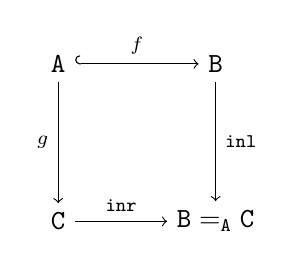
\begin{tikzpicture}
		\node (C) at (0,0) {$\C$};
		\node (BAC) at (2,0) {$\BAC$};
		\node (A) at (0,2) {$\A$};
		\node (B) at (2,2) {$\B$};
		\draw[right hook ->]  (A) to node [above] {\scriptsize $f$} (B);
		\draw[->]  (A) to node [left] {\scriptsize $g$} (C);
		\draw[->]  (B) to node [right] {\scriptsize $\inl$} (BAC);
		\draw[->]  (C) to node [above] {\scriptsize $\inr$} (BAC);
	\end{tikzpicture}
\]
also a set when $f$ is a monomorphism?

Thus to determine whether $\BAC$ is a set,
we need to access its identity types.  
We do this with an \emph{encode-decode} style proof.  

Roughly, a proof of this sort begins by guessing
what the identity types are.  That is,
for each $x$ and $y$ in $\BAC$, 
we define a type 
\[
	\code \from \BAC \to \BAC\to \Type
\]
so that $\code (x,y)$ serves as our guess  
as to what $x =_{\scriptsize \BAC} y$ actually is.  
Then we define functions
\[
	\type{ encode }_{ x , y } \from  ( x = y ) \to \code ( x , y ) 
	\text{ and }
	\type{ decode }_{ x , y } \from \code ( x , y ) \to ( x = y )
\]
for each $x$ and $y$ in $\BAC$.  
Hopefully, these are mutually inverse.

%%%%%%%%%%%%%%%%%%%%%%
%%%%%%%%%%%%%%%%%%%%%%
\pagebreak
\section{defining $\code$}

Let's try to define 
\[
	\code \from 
	\BAC \to \BAC \to \Type.
\]  
Note that $\code$ is a map from a pushout, 
so we define it using induction of higher types, 
as in Definition \ref{def:pushout}.
Hence we need three types schemes:
\begin{align*}
	\code(\inl(b)) & \from \BAC \to \Type \\
	\code(\inr(c)) & \from \BAC \to \Type \\
	\code( \ap_{\glue} (a) ) & \from \BAC \to \Type \\
\end{align*}
These schemes run through 
$a \tin A$, $b \tin B$, and $c \tin C$.  
They are also functions on the same coproduct!
To define $\code(\inl(b))$, 
we use higher induction which gives the type schemes:
\[
	\code(\inl(b),\inl(b')), \hspace{0.5em}
	\code(\inl(b),\inr(c')), \hspace{0.5em}
	\code(\inl(b),\ap_{\glue}(a')).
\]
Similarly, we define $\code(\inr(c))$ by
\[
	\code(\inr(c),\inl(b')), \hspace{0.5em}
	\code(\inr(c),\inr(c')) , \hspace{0.5em}
	\code(\inr(c),\ap_{\glue}(a')).
\]
and $\code(\glue(a))$ by 
\[
	\code(\ap_{\glue}(a),\inl(b')), \hspace{0.5em}
	\code(\ap_{\glue}(a),\inr(c')) , \hspace{0.5em} 
	\code(\ap_{\glue}(a),\ap_{\glue}(a')).
\]
The $\code$'s that have 
no $\ap_{\glue}$'s in the arguments 
correspond to our guesses
for the identity types.
The $\code$'s that have 
one $\ap_{\glue}$ in the arguments
give a pre- or post-composition
of paths.
The $\code$'s that have 
two $\ap_{\glue}$'s in the arguments  
ensure that this pre- and post-composition
action is coherent.
This fits together in a nice little 
diagram:
\[ % coherence diagram for code
	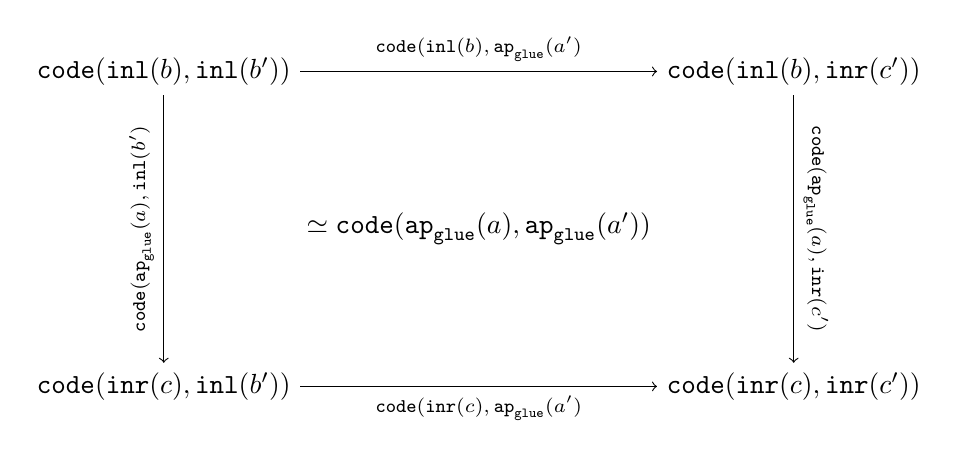
\begin{tikzpicture}
		\node (AA) at (0,0) 
			{ $ \simeq \type{ code } ( \ap_{\glue} ( a ) , \ap_{\glue} ( a' )  )$ }; 
		\node (BB) at (-4,2) 
			{ $ \type{ code } ( \inl( b ) , \inl( b' )  )$ }; 
		\node (BC) at (4,2) 
			{ $ \type{ code } ( \inl( b ) , \inr( c' )  )$ }; 
		\node (CB) at (-4,-2) 
			{ $ \type{ code } ( \inr( c ) , \inl( b' )  )$ }; 
		\node (CC) at (4,-2) 
			{ $ \type{ code } ( \inr( c ) , \inr( c' )  )$ }; 
		\draw [->] (BB) to 
			node 
				[above] 
				{\scriptsize $ \type{ code } ( \inl( b ) , \ap_{\glue} ( a' ) $ } 
			(BC);
		\draw [->] (BB) to 	
			node 
				[rotate=90,above] 
				{ \scriptsize $ \type{ code } ( \ap_{\glue} ( a ) , \inl( b' ) $ } 
			(CB);
		\draw [->] (BC) to 
			node 
				[rotate=-90, above] 
				{\scriptsize $\type{ code } ( \ap_{\glue} ( a ) , \inr( c' ) $} 
			(CC);
		\draw [->] (CB) to 	
			node 
				[below] 
				{ \scriptsize $ \type{ code } ( \inr( c ) , \ap_{\glue} ( a' ) $ } 
			(CC);
	\end{tikzpicture}
\]

%%%%%%%%%%%%%%%%%
\pagebreak
\subsection*{code( b,b')}

$\code \left( \inl ( b ) , \inl( b' ) \right)$ is the most complicated. 
In order to incorporate $\type{ refl }_b$ when $b$ is not in the image of $f$, 
we define this type to be the pushout of the span
\[
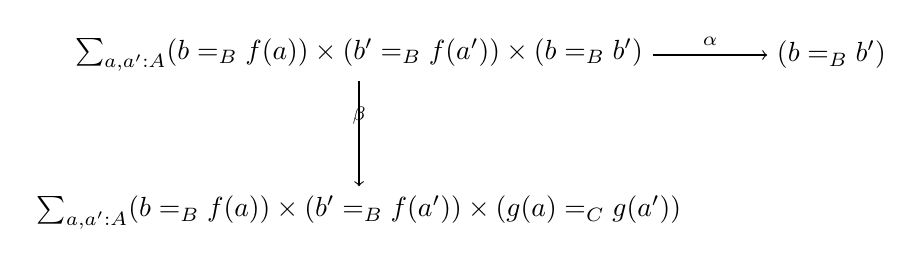
\begin{tikzpicture}
	\node (1) at (0,2) 
		{ $ \sum_{ a , a' : A } 
			( b =_B f ( a ) ) 
			\times ( b' =_B f ( a' ) ) 
			\times ( b =_B b' ) $ };
	\node (2) at (6,2) 
		{ $ ( b =_B b' ) $ };
	\node (3) at (0,0) 
		{ $ \sum_{ a , a' : A } 
			( b =_B f ( a ) ) 
			\times  (b' =_B f ( a' ) ) 
			\times ( g ( a ) =_C g ( a' ) ) $ };
	\draw [ -> ] (1) to 
		node [above] {\scriptsize $ \alpha $} 
		(2);
	\draw [ -> ] (1) to 
		node [above] {\scriptsize $ \beta $}
		(3);
\end{tikzpicture}
\]
Here, $ \alpha $ is a projection. Also,
$ \beta $ is a projection of the first
two factors and places $ \type{ ap }_g (p) $ 
in the third factor. This uses the injectivity of $f$
to get a $ p \tin a = a' $ if the upper left
is populated.

This is a proposition. 
Indeed, the span feet are propositions
and the only way for both to be populated
is if the apex is also populated.
But this would identify the 
left and right included elements
with a glue.

But this can be simplified via some case analysis. If $ (p,q,r) $ is in the upper left, then since we know that  we get a path $ q r p^{-1} : fa =_{\B} fa' $ which gives a $ \ell : a =_{\A} a' $ by injectivity of $ f $.  Thus we can $ \beta $-reduce $ fa' $ to $ fa $ which gives us $ (b=_{\B} fa) \times (b'=_{\B} fa) \times (b=_{\B} b') $.  Any witness to that has form $ (p,q',r) $ where $ q^{-1}p : b =_{\B} b' $ so since $ \B $ is a set, $ q^{-1}p = r $ so this $ (p,q',r) = (p,q',q^{-1}p) $.  Since the last factor depends on the first two, we can ignore it so we reduce the upper left further to $ (b=_{\B} fa) \times (b'=_{\B} fa) $.  But maybe a nicer thing to work with is $ (b=_{\B} fa) \times (b'=_{\B} fa') \times (a =_{\A} a') $.  Then $ \alpha $ assembles those maps into one of form $ b =_{\B} b' $ and $ \beta $ applies $ g $ to the last factor. That is, we can work instead with the pushout
\[
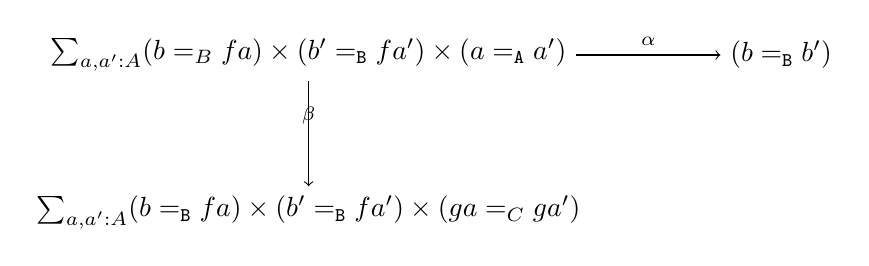
\begin{tikzpicture}
	\node (1) at (0,2) 
	{ $ \sum_{ a , a' : A } 
		( b =_B f  a ) 
		\times ( b' =_{\B} f  a' ) 
		\times ( a =_{\A} a' ) $ };
	\node (2) at (6,2) 
	{ $ ( b =_{\B} b' ) $ };
	\node (3) at (0,0) 
	{ $ \sum_{ a , a' : A } 
		( b =_{\B} f a ) 
		\times  (b' =_{\B} f a' ) 
		\times ( g a =_C g a' ) $ };
	\draw [ -> ] (1) to 
	node [above] {\scriptsize $ \alpha $} 
	(2);
	\draw [ -> ] (1) to 
	node [above] {\scriptsize $ \beta $}
	(3);
\end{tikzpicture}
\]
We can simplify this further due to the injectivity of $ f $.  The apex of the span can be boiled down to  
\[
	( b =_{\B} fa ) \times ( b' =_{\B} fa' ) \times ( a =_{\A} a' )  
\] 
is equivalent to 
\[
	( b =_{\B} fa ) \times ( b' =_{\B} fa ) 
\]
because if all three factors are populated, then we can $ \beta $-reduce $ a' $ to $ a $ and $ a =_{\A} a $ contains only $ \refl $ because $ \A $ is a set.  Thus, our pushout becomes
\[
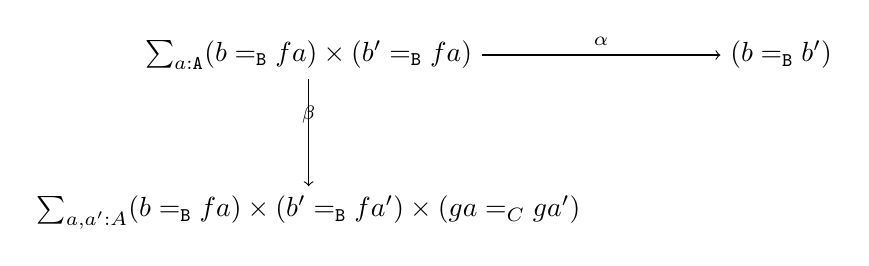
\begin{tikzpicture}
	\node (1) at (0,2) 
		{ $ \sum_{ a : \A } 
		( b =_\B f  a ) 
		\times ( b' =_{\B} f  a ) $} ; 
	\node (2) at (6,2) 
		{ $ ( b =_{\B} b' ) $ };
	\node (3) at (0,0) 
		{ $ \sum_{ a , a' : A } 
		( b =_{\B} f a ) 
		\times  (b' =_{\B} f a' ) 
		\times ( g a =_C g a' ) $ };
	\draw [ -> ] (1) to 
		node [above] {\scriptsize $ \alpha $} 
		(2);
	\draw [ -> ] (1) to 
		node [above] {\scriptsize $ \beta $}
		(3);
\end{tikzpicture}
\]


Later, when defining $ \decode $, we'll need to know what constructors this pushout has.  
\begin{itemize}
	\item $  \sum_{ a , a' : A } ( b =_B f  a ) \times ( b' =_{\B} f  a' ) \times ( a =_{\A} a' ) $.  Any witnesses $ (p,q,\ell) $ assembles into a path $ b =_{\B} b' $ so $ \alpha $ is injective.  Since $ \B $ is a set, this is a proposition.
	\item $  \sum_{ a , a' : A } ( b =_B f  a ) \times ( b' =_{\B} f  a' ) \times ( a =_{\A} a' ) $ .  This can only contain one element.  Indeed, suppose that $ (p,q,r) : ( b =_B f  a ) \times ( b' =_{\B} f  a' ) \times ( a =_{\A} a' ) $ and $ (p',q',r') : ( b =_B f  a'' ) \times ( b' =_{\B} f  a''' ) \times ( a'' =_{\A} a''' ) $ witness the lower left.  Then $ p $ and $ p' $ assemble to witness $ fa =_{\B} fa'' $. Similarly, $ q $ and $ q' $ assemble to witness $ fa' =_{\B} fa''' $. By injectivity of $ f $, we get than $ a =_{\A} a'' $ and $ a' =_{\A} a''' $.  So $ ( b =_B f  a'' ) \times ( b' =_{\B} f  a''' ) \times ( a'' =_{\A} a''' ) $ beta-reduces to $ ( b =_B f  a ) \times ( b' =_{\B} f  a'' ) \times ( a' =_{\A} a' ) $. This reduction identifies $ (p,q,r) $ and $ (p',q',r') $ because each factor is a set.  So the lower left is a proposition.
\end{itemize}

From this, it follows that both $ \alpha $ and $ \beta $are injections and so the pushout is a set by some older result (ask mike).  Anyway, depending on a few things we have different cases.
\begin{rmk} \label{rmk_code-bb-cases}
\begin{itemize}
	\item If $ p : b =_{\B} b' $ neither $ b,b' $ in the image of $ f $, then the only constructor of the pushout is $ \inl p $.
	\item If $ p : b =_{\B} b' $ and $ b $ is in the image of $ f $, then so is $ b' $.  Then the upper left is populated, which implies the lower left is and so the constructor are the elements included from the upper right and lower left which are then glued together.
	\item If $ b =_{\B} b' $ is empty is either $ b $ or $ b' $ are not in the image of $ f $ then both other corners are empty too, so no constructors.
	\item If $ b =_{\B} b' $ is empty, $ p: b =_{\B} fa $ and $ q : b' =_{\B} fa' $, then $ a =_{\A} a' $ must be empty, else we can prove $ b=_{\B}b' $. Hence upper right and upper left are empty.  So either $ ga =_{\C} ga' $ is empty or not.  If not, we get a constructor included from the lower left, else the pushout is empty.  
\end{itemize}
\end{rmk}

%
% commented out is discussion 
% to understand the pushout
%
%\begin{itemize}
%	\item Case 1---$ b,b' $ not in the image of $ f $, then only upper right can be non-empty, so $\type{ code } ( \inl( b ) , \inl( b' ) )$ is $ b =_{\B} b' $.
%	\item Case 2---$ b $ alone is in the image of $ f $. That is, for some $ a $, $ b =_{\B} fa $ is occupied, but for no $ a' $ is $ b=_{\B} fa' $ occupied.  It follows that $ b=_{\B} b' $ is empty, because otherwise $ b' =_{\B} b =_{\B} fa $.  Hence $\type{ code } ( \inl( b ) , \inl( b' ) )$ is empty.
%	\item Case3---$ b' $ alone is in the image of $ f $ mirrors case 2 by symmetry. Hence $\type{ code } ( \inl( b ) , \inl( b' ) )$ is empty.
%	\item Case 4---there exists $ a,a' : \A $ with $ b =_{\B} fa $ and $ b' =_{\B} fa' $.  There are two subcases here.
%	\begin{itemize}
%		\item Case 4a---$fa =_{\B} fa' $ is occupied. By injectivity of $ f $ we get $ \ell : a =_{\A} a' $ such that $ \ap_{f} \ell =_{\B} \ell $.  Given $ (p,q,r) $ in upper left, since $ \A $ is a set, we have that $ r =_{b =_{\B} b'} q^{-1}(\ap_{f}\ell) p $. Hence $ (p,q,r) =_{\text{upper left}} (p,q,q^{-1}(\ap_{f}\ell)p) $.  Now $ b=_{\B}b' $ is occupied and the witness must (since $ \B $ is a set) be $ \alpha (p,q,q^{-1}(\ap_{f}\ell) p) \coloneqq  q^{-1}\ell p$.  Moreover, $ \beta (p,q,q^{-1}(\ap_{f}\ell) p) \coloneqq = (p,q, \ap_{g} \ell) $. Hence this pushout has constructors $\inr (q^{-1}(\ap_{f}\ell)p) $, $ \inl (p,q, \ap_{g} \ell) $, and $ \glue (p,q,r) : \inr (q^{-1}(\ap_{f}\ell) p) = \inl (p,q, \ap_{g} \ell) $.  Are these all the constructors?  There are no more coming from $ b =_{\B} b' $ since $ \B $ is a set. To come from the bottom left, there must exist $ a'' , a''' : \A $ such that $ b =_{\B} fa'' $ and $ b' =_{\B} fa''' $. Then concatenating paths gives us $ fa =_{\B} fa'' $ and $ fa' =_{\B} fa''' $, which by injectivity of $ f $ means $ a =_{\A} a'' $ and $ a' =_{\A} a''' $. 
%		For this case, we assume that $ fa=_{\B}fa' $ is occupied, which now means that $ fa''=_{\B}fa''' $ and, by injectivity of $ f $, $ \ell' : a''=_{\A}a''' $.  Thus, in the lower left of the pushout square, there are two witnesses: $ (a,a',p,q,\ap_{f}\ell) $ and $ (a'',a''',p',q',\ap_{f}\ell') $. Now, since $ p' p^{-1} : fa =_{\B} fa'' $ and $ q' q^{-1} : fa' =_{\B} fa''' $, we get an $ \ell'' : a =_{\A} a'' $ and $ \ell''' : a' =_{\A} a''' $.  This gives $ \ell' \ell'' , \ell ''' \ell : a =_{\A} a''' $ which must commute because $ \A $ is a set.  Applying $ g $ to this square, we get a u
%		
%		{\color{red} are there any more elements being inl'ed from b=fa'' or b'=ba''' in this situation?}
%		\item Case 4b---$ fa =_{\B} fa' $ is not occupied
%	\end{itemize}
%\end{itemize}

%%%%%%%%%%%%%%%%%
\pagebreak
\subsection*{code (b,c)}

$
	\type{ code } \left( \inl( b ) , \inr( c' ) \right) \coloneqq
	\sum_{ a : A } ( b =_B f ( a ) ) \times ( c' =_C g ( a ) )
$
This is a proposition. 
Indeed, if there does not exist an $ a : A $ such that
$ b =_B f ( a )$ and $ c' =_C g ( a ) $
are both populated, then 
$ \type{ code } \left( \inl( b ) , \inr( c' ) \right) $ 
is empty. 
If there exists a single $a : A$ such that 
$ b =_B f ( a )$ and $ c' =_C g ( a ) $
are both populated, then 
because they are each equivalent to $ \type{ 1 }$,
$ \type{ code } \left( \inl( b ) , \inr( c' ) \right) $ 
is also equivalent to $ \type{ 1 }$.
If there is $a, a' : A$ such that
$ b =_B f ( a )$ and $ c' =_C g ( a ) $,
and also 
$ b =_B f ( a' )$ and $ c' =_C g ( a' ) $,
then the injectivity of $f$ and
$f ( a ) =_B b =_B f ( a' )$ 
implies that
$a =_A a'$
which also gives us that 
$ \type{ code } \left( \inl( b ) , \inr( c' ) \right) $ 
is equivalent to $ \type{ 1 }$.

%%%%%%%%%%%%%%%%%
\pagebreak
\subsection*{code (c,b)}

	$ \type{ code } \left( \inr( c ) , \inl( b' ) \right) \coloneqq \sum_{ a : A } ( c =_C g ( a ) ) \times ( b' =_B f ( a ) ) $
	This is a proposition by the same sort of argument from above.

%%%%%%%%%%%%%%%%%%
\pagebreak
\subsection*{code (c,c')}

	$ \type{ code } \left( \inr( c ) , \inr( c' ) \right) \coloneqq \sum_{ a , a' : A } ( c =_C g ( a ) ) \times ( c' =_C g ( a' ) ) \times ( f ( a ) =_B f ( a' ) ) $ 	
	The injectivity of $f$ gives us that 
	$ f ( a ) =_B f ( a' ) $
	imples that 
	$ a =_A a'$
	which in turn implies that
	$ g ( a ) =_C g ( a' )$,
	hence 
	$ c =_C c'$.
	Therefore, 
	$
	\type{ code } \left( \inr( c ) , \inr( c' ) \right) =	
	\left( c =_C c'  \right). 
	$
	Hence 
	$ \type{ code } \left( \inr( c ) , \inr( c' ) \right) $
	is a proposition.

%%%%%%%%%%%%%%%%%%%%
\pagebreak
\subsection*{code (b, glue a)}

These are all equivalences, hence by univalence
we define them as identity types. 
To show this, we show each is populated.

	$ 
	\type{ code } \left( \inl( b ) , \type{ ap }_{ \type{ glue } } ( a' ) \right) \colon \left( \type{ code } ( \inl( b ) , \inl( f ( a' ) ) ) = \type{ code } ( \inl( b ) , \inr( g ( a' ) ) ) \right) 
	$
	Because both sides of the identity type are propositions,
	to show that this equivalence holds
	it suffices to show that either
	$\type{ code } ( \inl( b ) , \inl( f ( a' ) ) )$
	and
	$\type{ code } ( \inl( b ) , \inr( g ( a' ) ) )$
	are both empty or both populated.
	This follows from post-composition with
	$ \type{ glue ( a' ) }$
	or its inverse.	

%%%%%%%%%%%%%%%%%%%%
\pagebreak
\subsection*{code (glue a, b)}

	$ 
	\type{ code } \left( \type{ ap }_{ \type{ glue } } ( a ) , \inl( b' ) \right) \colon
	\left(
	\type{ code } ( \inl( f ( a ) ) , \inl( b' ) ) =
	\type{ code } ( \inr( g ( a ) ), \inl( b' ) ) 
	\right)
	$
	This follows from a similar argument to that above, 
	with post-composition replaced with pre-composition.

%%%%%%%%%%%%%%%%%%%%
\pagebreak
\subsection*{code (c, glue a)}

	$ 
	\type{ code } \left( \inr( c ) , \type{ ap }_{ \type{ glue } } ( a' ) \right) \coloneqq
	\left( 
	\type{ code } ( \inr( c ) , \inl( f ( a' ) ) ) =
	\type{ code } ( \inr( c ) , \inr( g ( a' ) ) ) 
	\right) 
	$ 
	This follows from a similar argument.	

%%%%%%%%%%%%%%%%%%%%
\pagebreak
\subsection*{code (glue a , c)}

	$ 
	\type{ code } \left( \type{ ap }_{ \type{ glue } } ( a ) , \inr( c' ) \right) \coloneqq 
	\left( 
	\type{ code } ( \inl( f ( a ) ) , \inr( c' ) ) =
	\type{ code } ( \inr( g ( a ) ) , \inr( c' ) ) 
	\right) 
	$ 
	This follows from a similar argument.	

%%%%%%%%%%%%%%%%%%%%
\pagebreak
\subsection*{code (glue a, glue a')}

	$\type{ code } ( \type{ ap }_\type{ glue } ( a ) , \type{ ap }_\type{ glue } ( a' )  )$ is uniquely determined because
	everything involved is a proposition. 
	Because we have that the 1-cells 
	in the square are equalities,
	there is only a single way to commute.
	This single way is how we define our 2-cell.

%%%%%%%%%%%%%%%%%%%%%%
%%%%%%%%%%%%%%%%%%%%%%
\pagebreak
\section{defining $\encode$}

Now that $ \code $ is defined, we define maps between it and the identity types inside of $ B+_A C $. The first map we consider is encode, which is of type
\[
	\encode : 
		\prod_{x : \BAC} \prod_{y : \BAC} 
		(x=_{\BAC} y) \to  \code (x,y).
\]
What are the non-empty identity types in $ B+_A C $ that $ \encode $ must map from?  
\begin{itemize}
	\item for $ b,b' : B $ and $ p : b =_B b'  $, a path 
	\[
		\ap_{\inl}(p) : \inl (b) =_{\BAC} \inl (b')
	\]
	%
	\item for $ c,c' : C $ and $ q : c =_C c'  $, a path  
	\[
		\ap_{\inr}(q) : \inr (c) =_{\BAC} \inl (c') 
	\]
	%
	\item for $ a : A $, a path  
	\[
		\glue (a) : \inl(fa) =_{\BAC} \inr(ga)
	\] 
\end{itemize}

Thus it suffices to define the value of $ \encode $ for $ \ap_{\inl}(p) $, $ \ap_{\inr}(q) $, and $ \glue (a) $.  

Also, since we are mapping out of identity types, we can use path induction.

\begin{itemize}
	%___________
	\item Define 
	\[
		\encode \from (\inl (b) =_{\BAC} \inl (b)) \to \code (\inl(b),\inl(b))
	\] 
	by $ \refl_b \mapsto \ap_\inl (\type{refl_b})  $. Note that this $ \inl $ is coming from the span used to define $ \code(\inl(b),\inl(b)) $
	%____________
	\item Define 
	\[
		\encode \from (\inr (c) =_{\BAC} \inr (c)) \to \code (\inr(c),\inr(c))
	\] 
	by $ \refl_c \mapsto \ap_\inr (\refl_c)  $. Note that this $ \inr $ is coming from the span used to define $ \code(\inr(c),\inr(c)) $.
	%____________
	\item Define 
	\[
		\encode \from (\inl (fa) =_{\BAC} \inr (ga)) \to \code (\inl(fa),\inr(ga))
	\]
	by $ \glue (a) \mapsto ( \refl_{fa} , \refl_{ga}) $
\end{itemize}

%%%%%%%%%%%%%%%%%%%%%%
%%%%%%%%%%%%%%%%%%%%%%
\pagebreak
\section{defining $\decode$}

Define 
\[ % decode type
	\decode : 
	\prod_{x : \BAC} \prod_{y : \BAC} 
	\code (x,y) \to (x=_{\BAC} y).
\]
We can't use path induction because we are not mapping out of an
identity type. The general strategy will be to give values for $
\decode $ when feeding it the four different types of inputs--- $ b/b'
$, $ c/c' $, $ b/c $, and $ c/b $---as well as higher paths coming
from $ \glue $.  Of the former four, $ b/b' $ is the most difficult
because of the complicated definition for $ \code (\inl b , \inl b')
$.  When dealing with $ \glue $, we must ensure naturality, meaning
that there will be commuting diagrams to check.

\begin{itemize} 
	%____________
	\item The type
	\[
		\decode ( \inr c , \inr c') \from 
		\code ( \inr c , \inr c' ) \to ( c =_{\B +_{\A} \C}) c' )
	\]
	is given by $ p \mapsto \ap_{\inl} p $
	%____________
	\item The type 
	\[
		\decode ( \inl b , \inr c ) \from 
		\code ( \inl b , \inr c ) \to ( b =_{\B +_{\A} \C}) c )
	\]
	is trivial unless $ b = fa $ and $ c = ga $ hold. Define
	\[
		\decode ( \inl b , \inr c ) \from 
		\code ( \inl fa , \inr ga ) \to ( fa =_{\B +_{\A} \C}) ga )
	\]
	given by $ (p,q) \mapsto (\ap_{\inr} q^{-1}) (\glue a) (\ap_{\inl} p)$.
	%_______________
	\item The type 
	\[
		\decode ( \inr c , \inl b ) \from 
		\code ( \inr c , \inl b ) \to ( c =_{\B +_{\A} \C}) b )
	\]
	is trivial unless $ b = fa $ and $ c = ga $ hold. Define
	\[
		\decode ( \inr c , \inl b ) \from 
		\code ( \inr ga , \inl fa ) \to ( ga =_{\B +_{\A} \C}) fa )
	\]
	given by $ (q,p) \mapsto (\ap_{\inl} p^{-1}) (\glue a) (\ap_{\inr} q) $.
	%______________
	\item The type 
	\[
		\decode ( \inl b , \inl b' ) \from 
		\code ( \inl b , \inl b' ) \to ( b =_{\B +_{\A} \C}) b' )
	\]
	is more involved because $ \code ( \inl b , \inl b' ) $ is a pushout.  To define a map out of a pushout, define it on the constructors.  Hence, to define $ \decode ( \inl b , \inl b' ) $ we need to produce values for
	\begin{itemize}
		\item $ \decode ( \inl b , \inl b' ) (\inl p) $ for $ p : b =_{\B} b' $
		\item for each $ a,a' : \A $, define $ \decode ( \inl b , \inl b' ) (\inr (p,q,r)) $ for $ p : (b +_{\B} fa) $, $ q : (b' =_{\B} fa') $, and $ r : (ga =_{\C} ga') $, and
		\item $ \ap_{\decode ( \inl b , \inl b' )} (\glue a)  $ for $ a : \A $.
	\end{itemize}
	%______________
\end{itemize}

Now let's make the definitions depending on the four cases laid out in
Remark \ref{rmk_code-bb-cases}
\begin{itemize}
	\item Case 1. For $ p : b =_{\B} b' $, then define $ \decode (
\inl b , \inl b' ) (\inl p) = \ap_{\inl} \inl p$
	\item Case 2.  For $ \alpha (p,q,r) = p (\ap_f r) q^{-1} : b
=_{\B} b' $ and $ \beta (p,q,r) = (p,q,\ap_g r) : \sum_{a,a'} (b=b')
\times (b'=fa') \times (ga=ga') $, then define $ \decode (\inl b ,
\inl b') ( \inl p (\ap_f r) q^{-1}) $ to be $ \inl p (\ap_f r) q^{-1}
$.  Define $ \decode (\inl b , \inl b') ( \inr (p,q,\ap_g r) ) $ to be
$ (\inr q'^{-1})(\glue a')^{-1}(\ap_{g}r)(\glue a)(\inr p) $. This is
well defined because there is a $ \glue (p,q,r) $ connecting $ \inl (p
(\ap_f r) q^{-1}) $ to $ \inr (p,q,\ap_g r) $ in the $ \code (\inl b ,
\inl b') $ definition which we apply $ \decode $ to, identifying their
images.
	\item Case 3. Nothing to do, no constructors.
	\item Case 4. There is only one constructor, $ \inr (p,q,
\ap_g r) $.  Define $ \decode ( \inl b , \inl b') ( \inr (p,q, \ap_g
r) ) $ to be the path $ (\inr q'^{-1})(\glue a')^{-1}(\ap_{g}r)(\glue
a)(\inr p) $.
\end{itemize}

%\begin{itemize}
% \item $ \decode ( \inl b , \inl b' ) (\inl p) = \ap_{\inl} \inl p$
% \item $ \decode ( \inl b , \inl b' ) (\inr (a,a',p,q,s)) = %
% (\ap_{\inl} q) (\glue a'^{-1}) (\ap_{\inr} r) (\glue a) ( \ap_{\inl}
% p)$ % We need to check that this is well defined.  Here, that means
% ensuring that an element of $ \code (\inl b , \inl b') $ coming from
% % \[ % \sum_{a,a' : 'A} % (b =_{\B} fa) \times % (b' =_{\B} fa')
% \times % (b =_{\B} b')
% % \] % has the same output under $ \decode $ regardless if it travels
% via the pushout maps $ \alpha $ or $ \beta $.  Let's take an element
% % \[ % (a,a',p,q,r) : % \sum_{a,a' : 'A} % (b =_{\B} fa) \times % (b'
% =_{\B} fa') \times % (b =_{\B} b').
% % \]
% % \begin{itemize}
% % \item Under $ \alpha $, we have that $ \alpha (a,a',p,q,r) \coloneqq
% r $ which $ \decode (\inl b , \inl b') (\inl r) \coloneqq \ap_{\inl}
% r$.
% % \item Under $ \beta $, we have that $ \beta (a,a',p,q,r) \coloneqq
% (a,a',p,q, \ap_g s) $.  What is $ s $? Since $ r : (b =_{\B} b') $,
% then $ qrp^{-1} : fa =_{\A} f'a $. By the injectivity of $ f $, there
% exists $ s : a =_{\A} a' $.  Then $ \decode (\inl b , \inl b') $ sends
% this to
% % \[ % ( \ap_{inl} q )( \glue a'^{-1} )( \ap_{\inr} \ap_{g} s )( \glue
% a )( \ap_{\inl} p )
% % \] % {\color{red}ARE THESE EQUAL?}
% % \end{itemize}

To show \( \decode \)  is well defined, we must have that 
\[
  \decode ( \code (\inl fa,\inl b) ) = \decode ( \code (\inr ga, \inl b) ).
\]
Recall,
\[
  \code (\inr ga, \inl b) \coloneqq \Sigma_{x:\A} ( ga =_{\C} gx)
  \times ( b =_{\B} fx )
\]
and
\[
  \code ( \inl fa, \inl b)
\]
is the pushout of
\[
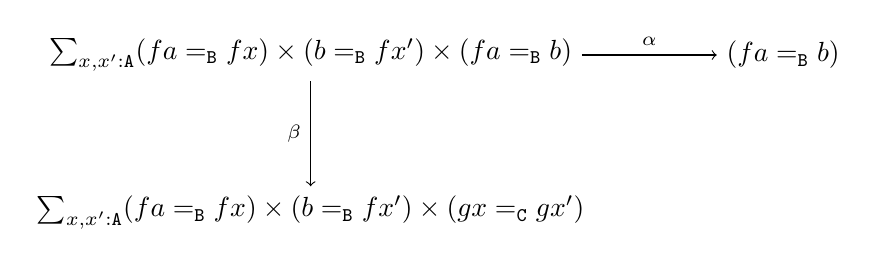
\begin{tikzpicture}
	\node (1) at (0,2) 
		{ $ \sum_{ x , x' : \A } 
			( fa =_{\B} fx ) 
			\times ( b =_{\B} fx' ) 
			\times ( fa =_{\B} b ) $ };
	\node (2) at (6,2) 
		{ $ ( fa =_{\B} b ) $ };
	\node (3) at (0,0) 
		{ $ \sum_{ x , x' : \A } 
			( fa =_{\B} fx ) 
			\times  (b =_{\B} fx' ) 
			\times ( gx =_{\C} gx') $ };
	\draw [ -> ] (1) to 
		node [above] {\scriptsize $ \alpha $} 
		(2);
	\draw [ -> ] (1) to 
		node [left] {\scriptsize $ \beta $}
		(3);
\end{tikzpicture}
\]
Clearly, \( \code ( \inr ga, \inl b ) \) it empty unless \( b =_{\B}
fa' \). The same can be said for \( \code ( \inl fa , \inl b ) \)
because the constructors of the pushout require either a populated \(
fa =_{\B} b \) or a populated \( b =_{\B} fx' \) for any \( x' : \A
\). So, we might as well assume that \( b =_{\B} fa \).  Why not \( b
=_{\B} fa' \) for some other \( a' : \A \)? I should think about this
later.

Now, we have that
\[
  \code (\inr ga, \inl fa) \coloneqq \Sigma_{x:\A} ( ga =_{\C} gx)
  \times ( fa =_{\B} fx )
\]
and
\[
  \code ( \inl fa, \inl fa)
\]
is the pushout of
\[
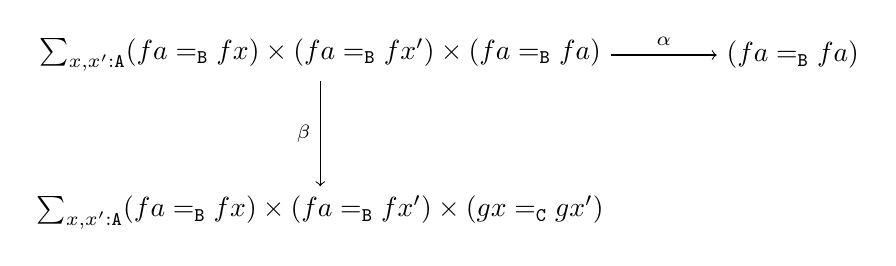
\begin{tikzpicture}
	\node (1) at (0,2) 
		{ $ \sum_{ x , x' : \A } 
			( fa =_{\B} fx ) 
			\times ( fa =_{\B} fx' ) 
			\times ( fa =_{\B} fa ) $ };
	\node (2) at (6,2) 
		{ $ ( fa =_{\B} fa ) $ };
	\node (3) at (0,0) 
		{ $ \sum_{ x , x' : \A } 
			( fa =_{\B} fx ) 
			\times  (fa =_{\B} fx' ) 
			\times ( gx =_{\C} gx') $ };
	\draw [ -> ] (1) to 
		node [above] {\scriptsize $ \alpha $} 
		(2);
	\draw [ -> ] (1) to 
		node [left] {\scriptsize $ \beta $}
		(3);
\end{tikzpicture}
\]
which should just be \( \{ \refl_{fa} \} \) since \( \B \) is a set.
It follows that \( \decode ( \code ( \inl fa , \inl fa ) ) \) maps \(
\refl_{fa} \) to \( (\refl_{fa}) \) as required.  We must now show
that \( \decode ( \code ( \inr ga , \inl fa ) ) \) is also \(
\refl_{fa} \).  But this follows from
\[
  \code ( \inr ga , \inl fa ) = (ga =_{\C} ga) \times ( fa _{\B} fa )
  = \{(\refl_{ga}, \refl_{fa})
\]
which is mapped via \( \decode \) to \( ( \ap_{\inl} \refl_{fa} ) (
\glue a ) ( \ap_{\inr} \refl_{ga} \), which is equal to \( \glue a \).
But since \( \glue a \) is contractible, it is homotopic to \( \refl_{fa} \).   




%%%%%%%%%%%%%
% end document
%%%%%%%%%%%%%




\end{document}
